\thispagestyle{fancy}
\fancyhead[R]{A.U 2025-2026}
\fancyhead[L]{Chapitre 4 : Sprint 2 -- Administration et mobilité}

\chapter{Sprint 2 : Administration à distance et mobilité}

\section*{Introduction}
Ce chapitre est consacré au \textbf{Sprint 2} du projet. Alors que le sprint précédent a
permis de construire le socle de supervision, ce sprint transforme la plateforme d'un
simple outil de \emph{visualisation} en un véritable outil d'\emph{administration}.

Il couvre quatre axes complémentaires : la détection automatique des anomalies à travers
un système d'alertes par seuils, l'exécution d'actions de maintenance à distance via des
connexions SSH sécurisées, l'automatisation des sauvegardes quotidiennes, et enfin la
mise à disposition de l'ensemble de ces fonctionnalités sur une application mobile
consommant la même API que le client web.

\section{Backlog du Sprint 2}
Après la définition des objectifs du Sprint 2, les \textit{User Stories} sélectionnées à
partir du \textit{Product Backlog} ont été décomposées en tâches techniques afin de
faciliter leur implémentation et leur suivi. Le tableau~\ref{tab:backlog-sprint2}
présente le backlog détaillé du Sprint 2.

\renewcommand{\arraystretch}{1.4}
\begin{longtable}{|>{\raggedright\arraybackslash}p{4.1cm}
                  |>{\raggedright\arraybackslash}p{7.7cm}
                  |>{\centering\arraybackslash}p{2.4cm}|}
\hline
\textbf{User Story} & \textbf{Tâches} & \textbf{Estimation} \\
\hline
\endfirsthead

\hline
\textbf{User Story} & \textbf{Tâches} & \textbf{Estimation} \\
\hline
\endhead

\hline
\multicolumn{3}{r}{\textit{Suite du tableau à la page suivante}} \\
\endfoot

\hline
\caption{Backlog du Sprint 2}
\label{tab:backlog-sprint2}
\endlastfoot

En tant que système, je veux générer une alerte lors du dépassement d'un seuil.
& Concevoir le modèle Mongoose \texttt{Alert}. & 1 \\
& Développer le service de génération d'alertes (\texttt{AlertService}). & 2 \\
& Externaliser les seuils dans la collection \texttt{Threshold}. & 1 \\
& Implémenter la détection des niveaux \texttt{WARNING} et \texttt{CRITICAL}. & 1 \\
& Éviter la génération d'alertes redondantes. & 2 \\
& Tester la génération. & 1 \\
\hline

En tant qu'administrateur, je veux être notifié par courrier électronique.
& Configurer le service d'envoi d'e-mails (Nodemailer / SMTP). & 1 \\
& Concevoir le modèle de message HTML de notification. & 2 \\
& Déclencher l'envoi lors de la génération d'une alerte. & 1 \\
& Tracer l'état d'envoi dans le document d'alerte. & 1 \\
& Tester la réception des notifications. & 1 \\
\hline

En tant qu'administrateur, je veux consulter et acquitter les alertes.
& Développer l'API de liste des alertes avec filtres. & 1 \\
& Développer l'API d'acquittement (\texttt{PUT .../acknowledge}). & 1 \\
& Développer l'API de résolution d'alerte. & 1 \\
& Réaliser l'interface de gestion des alertes. & 2 \\
& Tester les fonctionnalités. & 1 \\
\hline

En tant qu'agent, je veux détecter automatiquement les services actifs.
& Développer la fonction \texttt{detect\_active\_services()} en Python. & 2 \\
& Analyser la sortie de la commande \texttt{systemctl list-units}. & 1 \\
& Gérer les hôtes non-\texttt{systemd} sans interrompre la collecte. & 1 \\
& Ajouter le champ \texttt{services} au modèle \texttt{Server}. & 1 \\
& Persister la liste détectée à chaque cycle de collecte. & 1 \\
& Tester la détection. & 1 \\
\hline

En tant qu'administrateur, je veux redémarrer ou arrêter un service à distance.
& Développer le service d'exécution de commandes SSH (\texttt{node-ssh}). & 2 \\
& Implémenter la double vérification d'autorisation. & 2 \\
& Valider le nom de service par expression régulière. & 1 \\
& Développer les endpoints \texttt{restart-service} et \texttt{stop-service}. & 2 \\
& Gérer le cas particulier du gestionnaire de processus PM2. & 1 \\
& Vérifier le statut réel du service après l'action. & 2 \\
& Réaliser l'interface d'actions à distance. & 2 \\
& Tester les fonctionnalités. & 1 \\
\hline

En tant qu'administrateur, je veux redémarrer complètement un serveur.
& Développer l'endpoint de redémarrage du serveur. & 1 \\
& Implémenter la temporisation avant redémarrage. & 1 \\
& Mettre à jour le statut du serveur après l'action. & 1 \\
& Tester la fonctionnalité. & 1 \\
\hline

En tant qu'administrateur, je veux consulter le journal d'audit.
& Concevoir le modèle \texttt{AuditLog}. & 1 \\
& Développer le middleware de journalisation des actions. & 1 \\
& Envoyer une notification e-mail à chaque action d'administration. & 1 \\
& Développer l'API de consultation du journal. & 1 \\
& Réaliser l'interface de consultation. & 1 \\
& Tester la traçabilité. & 1 \\
\hline

En tant que système, je veux exécuter une sauvegarde quotidienne.
& Concevoir le modèle \texttt{Backup}. & 1 \\
& Mettre en place la tâche planifiée avec \texttt{node-cron}. & 1 \\
& Développer la procédure d'export de la base de données. & 2 \\
& Implémenter la vérification horaire des sauvegardes manquantes. & 1 \\
& Envoyer un e-mail de confirmation ou d'échec. & 1 \\
& Développer l'API et l'interface d'historique. & 1 \\
& Tester la planification. & 1 \\
\hline

En tant qu'administrateur, je veux accéder à la plateforme depuis mon téléphone.
& Mettre en place la navigation et la garde d'authentification (Expo Router). & 2 \\
& Développer le contexte d'authentification et la persistance du jeton. & 2 \\
& Réécrire la couche d'accès à l'API mobile. & 2 \\
& Développer l'écran de connexion. & 1 \\
& Développer le tableau de bord et le détail d'un serveur. & 2 \\
& Développer les écrans d'alertes et d'actions à distance. & 2 \\
& Implémenter le rafraîchissement automatique toutes les 5 secondes. & 1 \\
& Tester l'application sur appareil réel. & 1 \\
\hline

\end{longtable}

\section{Diagramme de cas d'utilisation du Sprint 2}
Dans cette section, nous présentons le diagramme de cas d'utilisation correspondant aux
fonctionnalités développées lors du deuxième sprint, tel qu'illustré dans la
figure~\ref{fig:uc-sprint2}.

\begin{figure}[H]
\centering
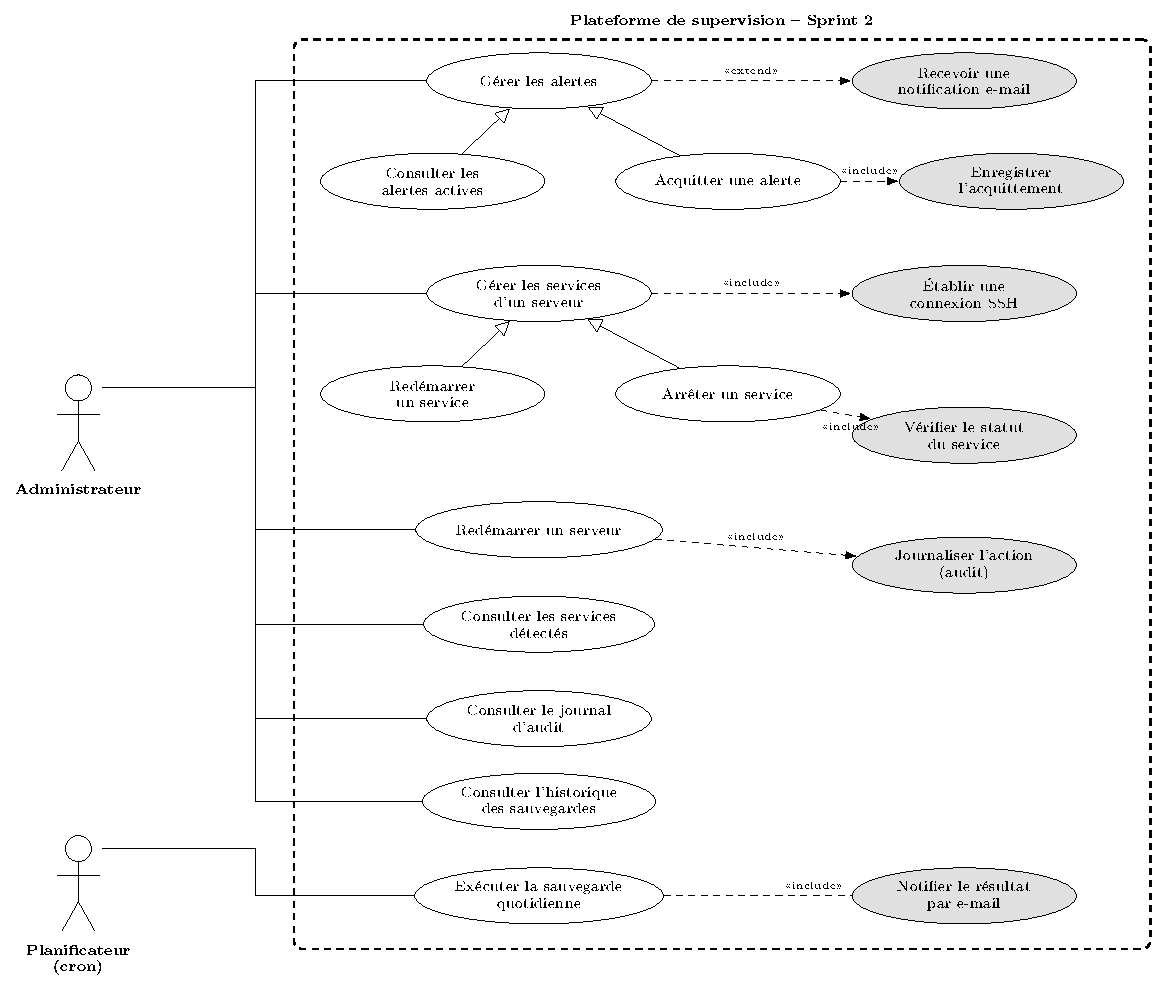
\includegraphics[width=\textwidth]{figures/uc-sprint2.pdf}
\caption{Diagramme de cas d'utilisation du Sprint 2}
\label{fig:uc-sprint2}
\end{figure}

\section{Services Web du Sprint 2}
Les services web développés durant ce sprint concernent la gestion des alertes,
l'exécution des actions à distance, la traçabilité des interventions et la consultation
des sauvegardes. Ils sont résumés dans le tableau~\ref{tab:ws-sprint2}.

\renewcommand{\arraystretch}{1.3}
\small
\begin{longtable}{|p{1.6cm}|>{\raggedright\arraybackslash}p{7.4cm}|p{5.4cm}|}
\hline
\textbf{Méthode} & \textbf{URL} & \textbf{Description} \\
\hline
\endfirsthead

\hline
\textbf{Méthode} & \textbf{URL} & \textbf{Description} \\
\hline
\endhead

\hline
\multicolumn{3}{r}{\textit{Suite du tableau à la page suivante}} \\
\endfoot

\hline
\caption{Liste des services web du Sprint 2}
\label{tab:ws-sprint2}
\endlastfoot

\multicolumn{3}{|c|}{\textbf{Gestion des alertes}} \\
\hline
\texttt{GET} & \texttt{/api/alerts} & Récupérer les alertes filtrées par statut, sévérité ou serveur. \\
\hline
\texttt{GET} & \texttt{/api/alerts/:alert\_id} & Consulter le détail d'une alerte. \\
\hline
\texttt{PUT} & \texttt{/api/alerts/:alert\_id/acknowledge} & Acquitter une alerte prise en charge. \\
\hline
\texttt{PUT} & \texttt{/api/alerts/:alert\_id/resolve} & Marquer une alerte comme résolue. \\
\hline
\texttt{GET} & \texttt{/api/alerts/stats/summary} & Obtenir les statistiques des alertes actives. \\
\hline
\texttt{POST} & \texttt{/api/alerts/bulk/acknowledge} & Acquitter plusieurs alertes en une seule opération. \\
\hline

\multicolumn{3}{|c|}{\textbf{Actions à distance sur les services}} \\
\hline
\texttt{GET} & \texttt{/api/remote-actions/}\allowbreak\texttt{:server\_id/}\allowbreak\texttt{services-status} & Vérifier l'état réel des services détectés sur un serveur. \\
\hline
\texttt{POST} & \texttt{/api/remote-actions/}\allowbreak\texttt{:server\_id/}\allowbreak\texttt{restart-service} & Redémarrer un service applicatif via SSH. \\
\hline
\texttt{POST} & \texttt{/api/remote-actions/}\allowbreak\texttt{:server\_id/}\allowbreak\texttt{stop-service} & Arrêter un service applicatif via SSH. \\
\hline
\texttt{POST} & \texttt{/api/remote-actions/}\allowbreak\texttt{:server\_id/}\allowbreak\texttt{start-service} & Démarrer un service applicatif via SSH. \\
\hline

\multicolumn{3}{|c|}{\textbf{Actions à distance sur le serveur}} \\
\hline
\texttt{POST} & \texttt{/api/remote-actions/}\allowbreak\texttt{:server\_id/}\allowbreak\texttt{restart} & Redémarrer complètement un serveur via SSH. \\
\hline
\texttt{POST} & \texttt{/api/remote-actions/}\allowbreak\texttt{:server\_id/}\allowbreak\texttt{shutdown} & Arrêter un serveur avec motif d'intervention. \\
\hline
\texttt{GET} & \texttt{/api/remote-actions/}\allowbreak\texttt{:server\_id/}\allowbreak\texttt{audit-log} & Consulter le journal d'audit des actions d'un serveur. \\
\hline

\multicolumn{3}{|c|}{\textbf{Gestion des sauvegardes}} \\
\hline
\texttt{GET} & \texttt{/api/backups} & Récupérer l'historique des sauvegardes réalisées. \\
\hline
\texttt{GET} & \texttt{/api/backups/:id} & Consulter le détail d'une sauvegarde. \\
\hline

\end{longtable}
\normalsize

\section{Les cas d'utilisation du Sprint 2}

\subsection{Cas d'utilisation : « Redémarrer un service à distance »}
Ce cas d'utilisation constitue la fonctionnalité la plus sensible de la plateforme,
puisqu'elle permet d'exécuter une commande privilégiée sur un serveur distant depuis
l'interface. Elle fait donc l'objet d'un dispositif de sécurité renforcé.

\subsubsection*{Description textuelle}

\renewcommand{\arraystretch}{1.4}
\begin{longtable}{|p{3.0cm}|>{\raggedright\arraybackslash}p{11.4cm}|}
\hline
\textbf{Acteurs} & Administrateur \\
\hline
\textbf{Objectif} & Permettre à l'administrateur authentifié de redémarrer un service
applicatif sur un serveur supervisé, directement depuis l'interface web ou mobile, sans
ouvrir manuellement de session SSH, tout en garantissant la traçabilité de l'action. \\
\hline
\textbf{Pré-condition} & L'administrateur est authentifié et dispose du rôle
\texttt{admin}. Le serveur cible possède des identifiants SSH renseignés
(\texttt{ip\_address}, \texttt{ssh\_username}, \texttt{ssh\_password}). Le service visé
figure parmi ceux détectés par l'agent. \\
\hline
\textbf{Scénario principal} &
\begin{enumerate}[leftmargin=*, nosep]
  \item L'administrateur sélectionne un serveur dans le module d'actions à distance.
  \item Le système affiche la liste des services réellement détectés sur ce serveur,
        accompagnés de leur état courant.
  \item L'administrateur clique sur le bouton « Redémarrer » du service concerné.
  \item Le système vérifie la validité du jeton JWT.
  \item Le système vérifie en base de données que l'utilisateur possède le rôle
        administrateur.
  \item Le système valide le nom du service par expression régulière afin de prévenir
        toute injection de commande.
  \item Le système établit une connexion SSH vers le serveur cible.
  \item Le système exécute la commande \texttt{sudo systemctl restart <service>}.
  \item Le système vérifie l'état réel du service au moyen de
        \texttt{systemctl is-active}.
  \item Le système journalise l'action dans le journal d'audit et envoie une
        notification par courrier électronique.
  \item Le système retourne le résultat accompagné du statut vérifié.
\end{enumerate} \\
\hline
\textbf{Scénarios alternatifs} &
\textit{A1 : Jeton absent ou expiré}
\begin{enumerate}[leftmargin=*, nosep]
  \item Le système renvoie une erreur 401 et invite l'utilisateur à se reconnecter.
\end{enumerate}
\textit{A2 : Utilisateur non administrateur}
\begin{enumerate}[leftmargin=*, nosep]
  \item Le système renvoie une erreur 403 et refuse l'exécution.
\end{enumerate}
\textit{A3 : Identifiants SSH incomplets}
\begin{enumerate}[leftmargin=*, nosep]
  \item Le système renvoie une erreur 400 en précisant les champs manquants.
\end{enumerate}
\textit{A4 : Échec de la commande distante}
\begin{enumerate}[leftmargin=*, nosep]
  \item Le système récupère le flux d'erreur, journalise l'échec et le retourne à
        l'administrateur.
\end{enumerate}
\textit{A5 : Cas particulier de PM2}
\begin{enumerate}[leftmargin=*, nosep]
  \item PM2 n'étant pas un service \texttt{systemd}, le système exécute la commande
        \texttt{pm2 restart all} et vérifie l'état via \texttt{pm2 jlist}.
\end{enumerate} \\
\hline
\caption{Cas d'utilisation : Redémarrer un service à distance}
\label{tab:cu-restart}
\end{longtable}

\subsubsection*{Diagramme de séquence système}
La figure~\ref{fig:seq-sys-restart} illustre les interactions entre l'administrateur et
le système lors de l'exécution d'une action à distance.

\begin{figure}[H]
\centering
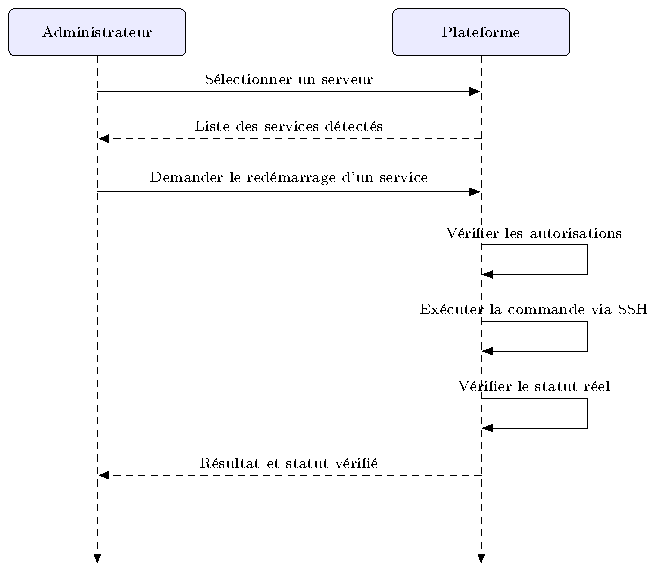
\includegraphics[width=0.9\textwidth]{figures/seq-sys-restart.pdf}
\caption{Diagramme de séquence système du cas d'utilisation « Redémarrer un service à distance »}
\label{fig:seq-sys-restart}
\end{figure}

\subsubsection*{Diagramme de séquence objet}
La figure~\ref{fig:seq-obj-restart} détaille les interactions entre les composants
internes du système lors de l'exécution d'une action à distance.

\begin{figure}[H]
\centering
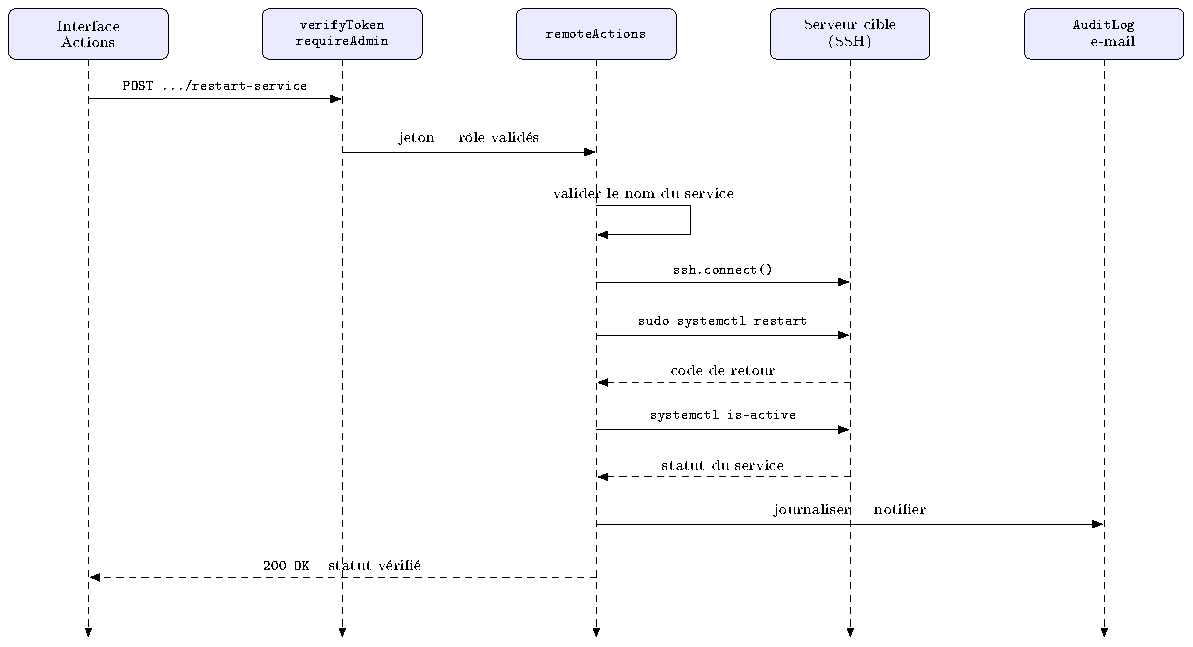
\includegraphics[width=\textwidth]{figures/seq-obj-restart.pdf}
\caption{Diagramme de séquence objet du cas d'utilisation « Redémarrer un service à distance »}
\label{fig:seq-obj-restart}
\end{figure}

\subsection{Cas d'utilisation : « Générer et notifier une alerte »}
Ce cas d'utilisation décrit le mécanisme automatique de détection des anomalies, qui
constitue le cœur de la valeur ajoutée de la plateforme.

\subsubsection*{Description textuelle}

\renewcommand{\arraystretch}{1.4}
\begin{longtable}{|p{3.0cm}|>{\raggedright\arraybackslash}p{11.4cm}|}
\hline
\textbf{Acteurs} & Système (traitement automatique), Administrateur (destinataire) \\
\hline
\textbf{Objectif} & Détecter automatiquement le dépassement d'un seuil de consommation
de ressources sur un serveur supervisé, générer l'alerte correspondante et en informer
immédiatement l'administrateur. \\
\hline
\textbf{Pré-condition} & Une métrique vient d'être reçue et persistée. Les seuils sont
configurés dans la base de données. \\
\hline
\textbf{Scénario principal} &
\begin{enumerate}[leftmargin=*, nosep]
  \item Le système reçoit une nouvelle métrique de l'agent.
  \item Le service de calcul de statut compare successivement les valeurs de CPU, RAM et
        disque aux seuils configurés.
  \item Un dépassement est détecté (\texttt{WARNING} à 80\,\%, \texttt{CRITICAL} à
        90\,\%).
  \item Le système vérifie qu'une alerte identique n'est pas déjà active sur ce serveur
        afin d'éviter les doublons.
  \item Le système crée un document \texttt{Alert} avec la sévérité, la métrique
        concernée, la valeur mesurée, le seuil dépassé et un message explicite.
  \item Le système envoie une notification par courrier électronique à l'administrateur.
  \item Le système marque l'alerte comme notifiée et diffuse la mise à jour aux clients
        connectés.
  \item L'alerte apparaît dans la liste des alertes actives sur l'interface web et
        mobile.
\end{enumerate} \\
\hline
\textbf{Scénarios alternatifs} &
\textit{A1 : Alerte déjà active}
\begin{enumerate}[leftmargin=*, nosep]
  \item Aucune nouvelle alerte n'est créée ; l'alerte existante reste active.
\end{enumerate}
\textit{A2 : Retour à la normale}
\begin{enumerate}[leftmargin=*, nosep]
  \item Les valeurs repassent sous les seuils : les alertes actives du serveur sont
        automatiquement résolues.
\end{enumerate}
\textit{A3 : Échec de l'envoi du courrier électronique}
\begin{enumerate}[leftmargin=*, nosep]
  \item L'alerte est tout de même enregistrée ; l'échec d'envoi est journalisé.
\end{enumerate} \\
\hline
\caption{Cas d'utilisation : Générer et notifier une alerte}
\label{tab:cu-alerte}
\end{longtable}

\subsubsection*{Diagramme de séquence objet}
La figure~\ref{fig:seq-obj-alerte} illustre les interactions internes lors de la
génération d'une alerte.

\begin{figure}[H]
\centering
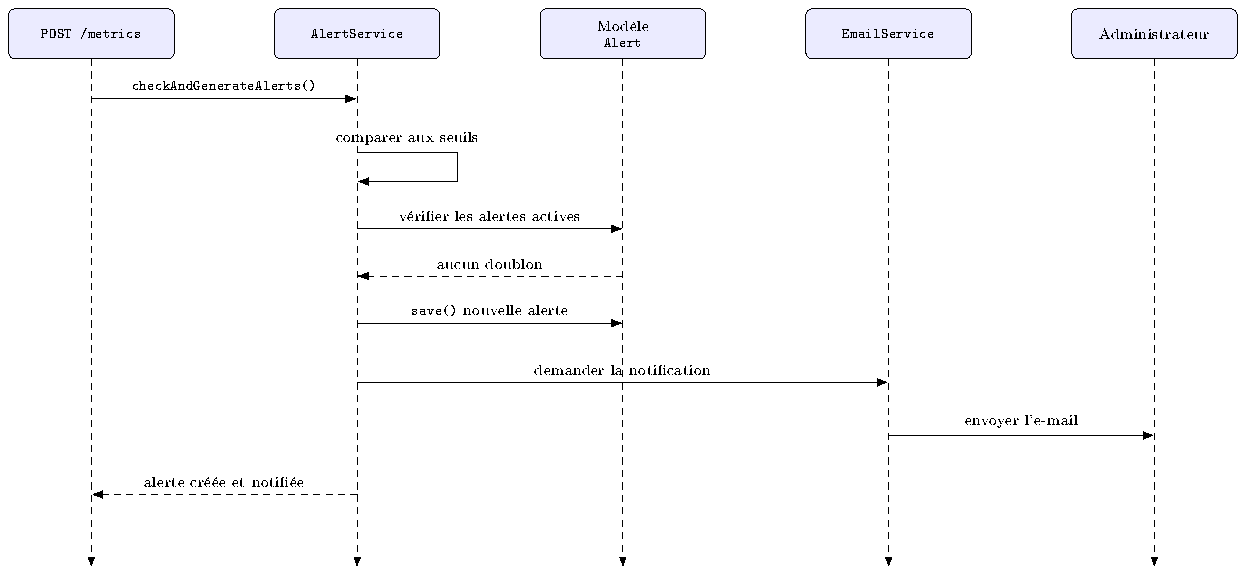
\includegraphics[width=\textwidth]{figures/seq-obj-alerte.pdf}
\caption{Diagramme de séquence objet du cas d'utilisation « Générer et notifier une alerte »}
\label{fig:seq-obj-alerte}
\end{figure}

\section{Détection automatique des services}
Une contrainte majeure identifiée lors de la conception concernait la gestion des
services applicatifs : imposer une liste fixe de services aurait limité la plateforme à
un ensemble prédéfini, incompatible avec un parc hétérogène.

La solution retenue repose sur une \textbf{détection dynamique} réalisée par l'agent
Python. À chaque cycle de collecte, celui-ci exécute la commande présentée dans
l'extrait~\ref{lst:systemctl}, analyse la sortie obtenue et transmet au backend la liste
des unités actives, débarrassées de leur suffixe.

\begin{figure}[H]
\centering
\fbox{\parbox{0.92\textwidth}{\ttfamily\small
systemctl list-units -{}-type=service -{}-state=active -{}-no-pager -{}-plain
}}
\caption{Commande de détection des services actifs}
\label{lst:systemctl}
\end{figure}

Cette liste est persistée dans le champ \texttt{services} du document \texttt{Server},
puis exploitée de deux manières complémentaires :

\begin{itemize}[label=\ding{43}]
  \item l'interface n'affiche que les services \emph{réellement présents} sur le serveur
        sélectionné, évitant toute action sur un service inexistant ;
  \item le backend s'appuie sur cette liste comme \emph{liste blanche} avant d'exécuter
        une commande, renforçant ainsi la protection contre l'injection de commandes.
\end{itemize}

Le traitement est conçu pour ne jamais interrompre la collecte : si la commande échoue —
par exemple sur un hôte dépourvu de \texttt{systemd} — la liste retournée est simplement
vide et les métriques continuent d'être transmises normalement.

\section{Réalisation du Sprint 2}

\begin{itemize}[label=\ding{220}]
\item \textbf{Gestion des alertes :}
\end{itemize}
La figure~\ref{fig:real-alertes} illustre l'interface de gestion des alertes.
L'administrateur y consulte l'ensemble des alertes actives avec leur sévérité, le serveur
concerné, la métrique en cause et la valeur mesurée. Chaque alerte peut être acquittée
d'un simple clic.

\begin{figure}[H]
    \centering
    \includegraphics[width=0.9\textwidth]{Image/real-alertes.png}
    \caption{Interface de gestion des alertes}
    \label{fig:real-alertes}
\end{figure}

\begin{itemize}[label=\ding{220}]
\item \textbf{Notification par courrier électronique :}
\end{itemize}
La figure~\ref{fig:real-email} présente le courrier électronique reçu automatiquement par
l'administrateur lors du dépassement d'un seuil. Il précise le serveur concerné, la
métrique en cause, la valeur mesurée et le seuil franchi.

\begin{figure}[H]
    \centering
    \includegraphics[width=0.8\textwidth]{Image/real-email-alerte.png}
    \caption{Notification d'alerte par courrier électronique}
    \label{fig:real-email}
\end{figure}

\begin{itemize}[label=\ding{220}]
\item \textbf{Actions à distance sur les services :}
\end{itemize}
La figure~\ref{fig:real-actions} illustre le module d'actions à distance. Après sélection
d'un serveur, l'administrateur visualise les services réellement détectés avec leur état
courant, et dispose pour chacun des boutons « Redémarrer » et « Arrêter ».

\begin{figure}[H]
    \centering
    \includegraphics[width=0.9\textwidth]{Image/real-actions.png}
    \caption{Module d'actions à distance sur les services}
    \label{fig:real-actions}
\end{figure}

\begin{itemize}[label=\ding{220}]
\item \textbf{Journal d'audit :}
\end{itemize}
La figure~\ref{fig:real-audit} présente le journal d'audit. Chaque action d'administration
y est enregistrée avec son auteur, sa cible, la commande exécutée, l'horodatage et le
résultat obtenu, garantissant une traçabilité complète des interventions.

\begin{figure}[H]
    \centering
    \includegraphics[width=0.9\textwidth]{Image/real-audit.png}
    \caption{Journal d'audit des actions à distance}
    \label{fig:real-audit}
\end{figure}

\begin{itemize}[label=\ding{220}]
\item \textbf{Historique des sauvegardes :}
\end{itemize}
La figure~\ref{fig:real-backups} illustre l'interface de consultation des sauvegardes.
L'administrateur y suit l'exécution quotidienne planifiée à minuit, avec pour chaque
sauvegarde son horodatage, sa taille et son statut.

\begin{figure}[H]
    \centering
    \includegraphics[width=0.9\textwidth]{Image/real-backups.png}
    \caption{Historique des sauvegardes automatisées}
    \label{fig:real-backups}
\end{figure}

\begin{itemize}[label=\ding{220}]
\item \textbf{Application mobile :}
\end{itemize}
La figure~\ref{fig:real-mobile} présente les principaux écrans de l'application mobile :
connexion, tableau de bord, gestion des alertes et actions à distance. L'application
consomme la même API REST que le client web et se rafraîchit automatiquement toutes les
5 secondes, permettant à l'administrateur d'intervenir en situation de mobilité.

\begin{figure}[H]
    \centering
    \includegraphics[width=0.95\textwidth]{Image/real-mobile.png}
    \caption{Écrans de l'application mobile}
    \label{fig:real-mobile}
\end{figure}

\section*{Conclusion}
Ce chapitre a présenté les fonctionnalités développées lors du Sprint 2. Celui-ci a
permis de doter la plateforme d'un système d'alertes automatique par seuils avec
notification par courrier électronique, d'un module d'actions à distance sécurisé par
double vérification et intégralement tracé, d'une détection dynamique des services
applicatifs, d'un mécanisme de sauvegarde quotidienne automatisée, ainsi que d'une
application mobile offrant les mêmes fonctionnalités en situation de mobilité.

À l'issue de ce sprint, l'application de supervision est fonctionnellement complète. Les
deux sprints suivants portent sur son industrialisation selon une démarche DevSecOps.
